\selectlanguage{english}
\chapter{The CMS detector at LHC}
\label{Chapter2}
%SourceDoc tesi.tex

\section{The Large Hadron Collider}
Approved in the early '90s and started up in the 2008, the \textit{Large Hadron Collider} is currently the world's largest and most powerful particle accelerator. \\
Its main purpose is to help in testing the predictions of different theories of particle physics, including the search of the Higgs boson and the dark matter. \\
Built at a mean depth of 100m, beneath France-Switzerland border near Geneva, in the tunnel formerly used to house the Large Electron-Positron collider (LEP), the LHC  of a 26.7km ring of superconducting magnets with a number of accelerating structures to boost the energy of the particles along the way. It is not a perfect circle: it is made of eight arcs and eight 'insertions'. The arcs are long 106.9m with a curvature of 2.84km containing 1232 superconductive dipoles. The LHC dipoles use Niobium-Titanium (NbTi) cables at a temperature of 1.9K, pumping superfluid helium into the magnet system, where they become superconducting; a current of 11850A flows in the dipoles to create the high magnetic field of 8.33 T required to bend the beams around the ring. 
%due to geological consideration, it has a slight gradient of 1.4\% and its depth varies between 150m (under the Jura) and 50m (towards lake Geneva ). 
The insertions instead consist of a long straight section of 528m plus two (one at each end) transition regions. They contains the radiofrequency cavities to increase beam energy (0.5 MeV per period): there are eight cavities per beam, each delivering 2MV (an accelerating field of 5MV/m) at 400MHz operating at 4.5K. Particular kind of insertion are quadrupoles, special magnets used to focus the beam down to the smallest possible size at the collision points: there 392 quadrupoles in LHC. \\
In the LHC each particle beam is accelerated up to 6.5 TeV (7 TeV is the designed energy not yet reached) but it is the last element of the accelerating chain. \\
The proton beam is created by using an electric field to pull the electrons from hydrogen atoms and start the acceleration. Protons are injected into the PS Booster (PSB) at an  energy of 50 MeV from Linac2 (Linear Accelerator 2). The booster comprises four superposed rings: this is because at low energy intensity, the quality of the beams suffers from the repulsive forces between particles. By splitting up the injected beam this effect gets reduced. Once the beam reaches the energy of 1.4 GeV it is extracted and injected into Proton Synchrotron (PS). With a circumference of 628 m, the PS accelerates the beams up to 26 GeV when they are extracted and sent to the Super Proton Synchrotron (SPS). Built in the '70, the SPS has a length of 7 km. The beam is injected at 26 GeV, ramped up to 450 GeV and extracted to the LHC. At the SPS, the boson W and Z were discovered and this led Rubbia and Simon van der Meer to win the Nobel prize. In \figurename~\ref{Cern-Accelerator-Complex}  a complete scheme of the accelerator chain of the LHC.\\
\begin{figure}[htbp]
\centering
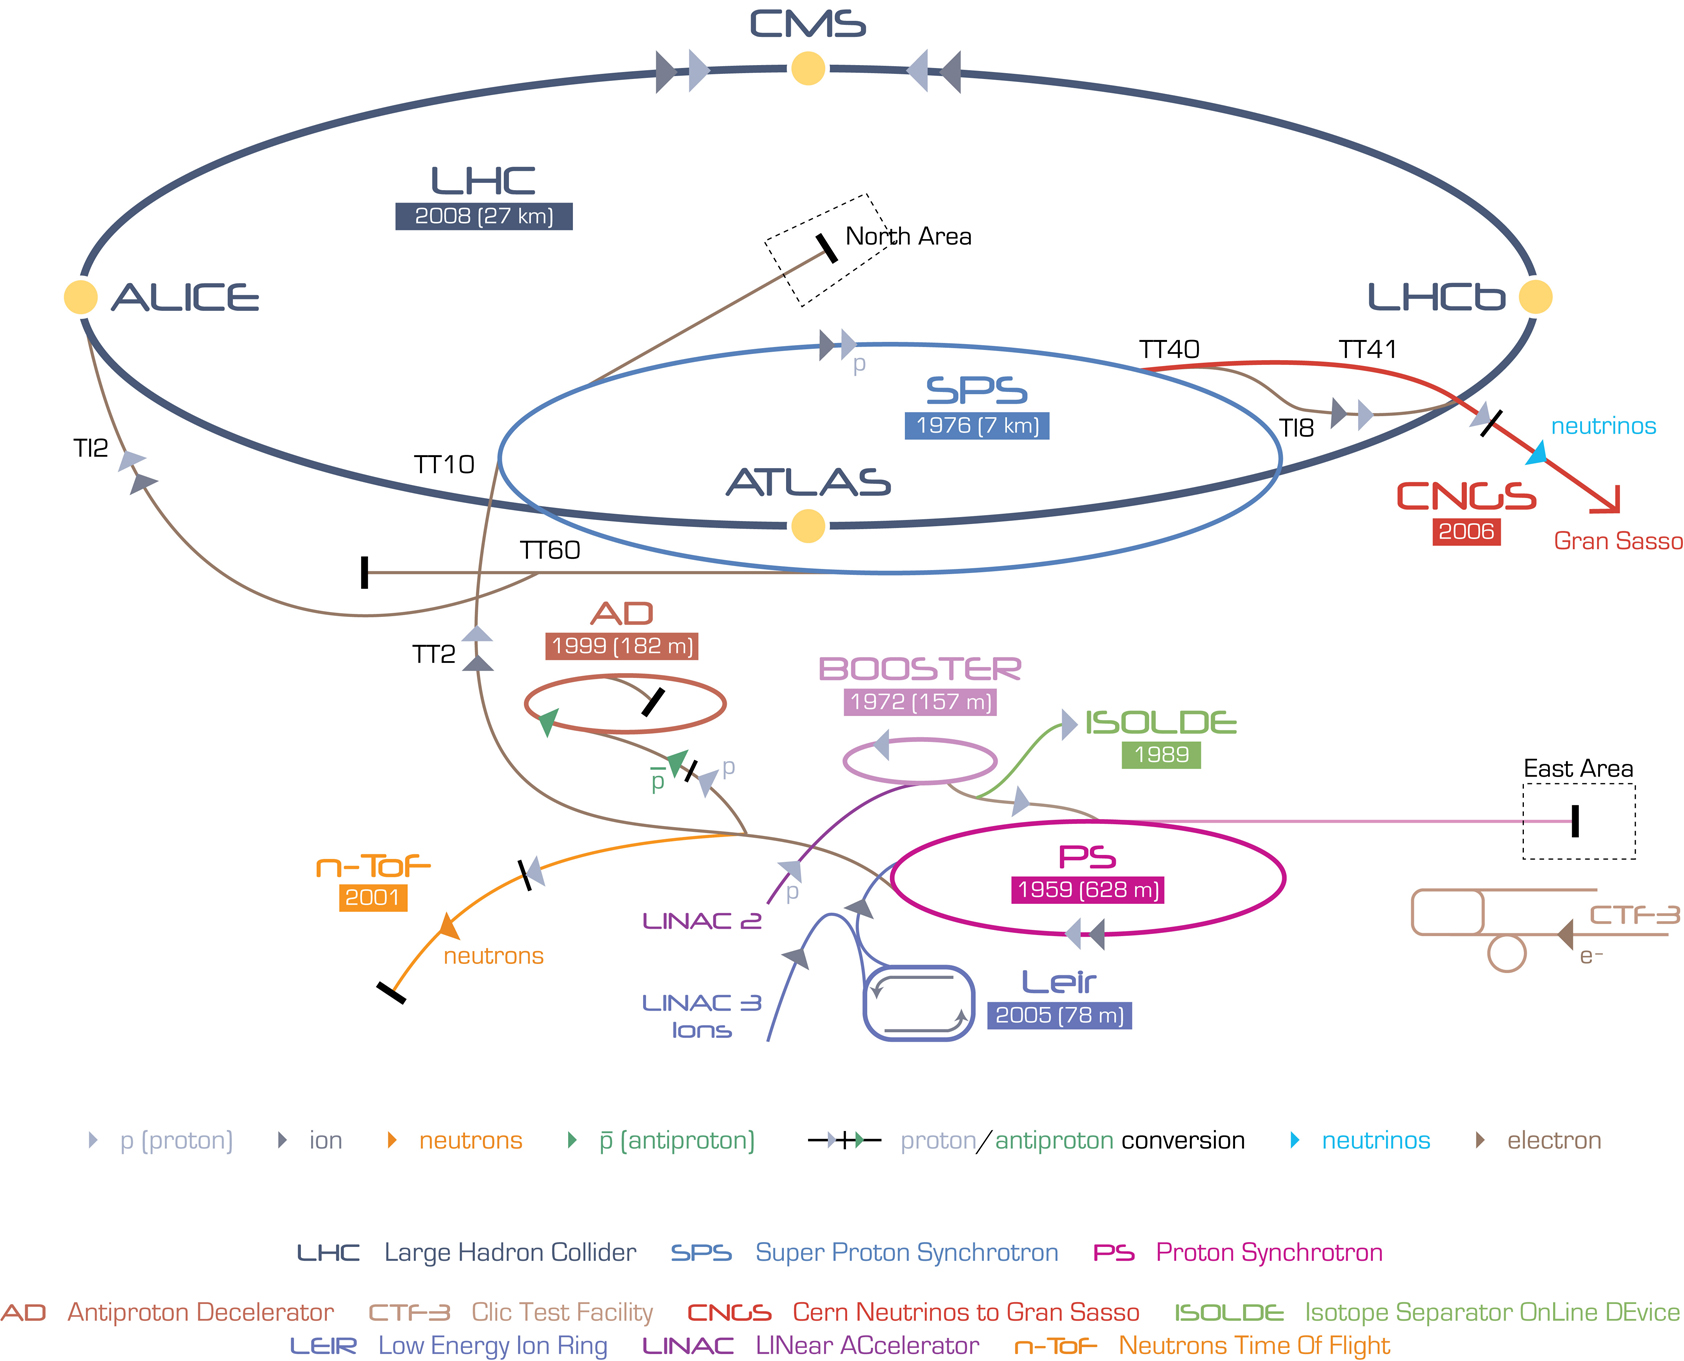
\includegraphics[width=0.65\textwidth]{Images/Cern-Accelerator-Complex}
\caption{Accelerator scheme at CERN.}
\label{Cern-Accelerator-Complex}
\end{figure}
Once the energy-working point is reached, the beams are made to collide at four locations around the LHC, corresponding to the position of four particles detectors: ALICE (\emph{A Large Ion Collider Experiment}), ATLAS (\emph{A Toroidal LHC ApparatuS}), CMS (\emph{Compact Muon Solenoid}) and LHCb (\emph{Large Hadron Collider beauty}). In addition to these, there are other three experiment installed at the LHC: TOTEM (\textit{TOTal Elastic and diffractive cross section Measurement}) installed close to CMS, MoEDAL (\textit{Monopole and Exotics Detector at the LHC}) close to LHCb and LHCf (\textit{Large Hadron Collider forward}) near ATLAS. \\
The beams at LHC have a bunch structure as a direct consequence of the radio frequency acceleration scheme. Protons can only be accelerated when the RF field has the correct orientation when particles pass through an accelerating cavity. Under nominal operating conditions, each proton beam has 2808 bunches, with each bunch containing about $10^{11}$ protons. The bunch size is not constant around the ring getting squeezed as much as possibile around the interaction points in order to increase the probability of collision. They measure a few centimetres long and a millimetre wide when they are far from a collision point; as the bunches approach  the collision points, they are squeezed to about $20\ \mu m$. LHC uses a bunch spacing of 25 ns (or 7.5 m) corresponding to a frequency of 40 MHz. \\
High frequency and small beam section, let to increase the number of events, the so call \textit{rate}, defined as:
\begin{equation}
\mathcal{R} = \sigma \times \mathcal{L}
\label{rate}
\end{equation}
In \ref{rate}, $\sigma$ represents the cross section of a particular event and $\mathcal{L}$ is the luminosity:
\begin{equation}
\mathcal{L} = \frac{f k_{B} N^{2}_{P}}{4 \pi \sigma_{x} \sigma_{y}}
\label{luminosity}
\end{equation}
where f is the frequency, $k_{B}$ the number of bunch and $N_{P}$ the number of proton in each bunch, $\sigma_{x}$ and $\sigma_{y}$ instead are the transversal sizes of the bunch at interaction point. \\
In \tablename~\ref{LHC_parameteres} are reported the designed LHC parameters and the ones reached at the end of RunII in 2018.
\begin{table}[htbp]	
	\begin{center}
		\begin{tabular}{p{6cm}*{3}{c}}
			\hline   &  & Design & 2018  \\
			\hline
			\hline
			\bfseries Centre of mass energy & \emph{E} & 14 TeV & 13 TeV \\
			\hline
			\bfseries Luminosity & \emph{L} & 10$^{34}$ cm$^{-2}$s$^{-1}$ & --- \\
			\hline
			\bfseries Time spacing &  & 25 ns & 25 ns\\
			\hline
			\bfseries Num. of bunches& \emph{k$_{B}$} & 2808 & ---\\
			\hline
			\bfseries Num. protons per bunch & \emph{N$_{p}$} & 1.15$\times$10$^{11}$ & ---\\
			\hline
			\hline
		\end{tabular}
	\end{center}
	\caption{LHC parameters}
	\label{LHC_parameteres}
\end{table}

\section{The Compact Muon Solenoid}
CMS, \textit{Compact Muon Solenoid}, is one of the four biggest experiment installed at LHC: it is a general-purpose detector designed to cover the widest possible range of physics at LHC, from precision measurements of the Higgs boson to searches for new physics beyond the Standard Model. \\
It is is a 21.6 m long cylinder with a diameter of 14.6 m and a total weight of 12500 tons. Its main feature is the cylindrical coil of superconducting cable that generates a magnetic field of 4 T. The importance to have a huge magnetic field is linked with the necessity to measure as precise as can, the momentum of the particles:
\begin{equation}
p[TeV] = 0.3 \cdot B[T] \cdot R[km]
\end{equation}
with the relative error  $\sigma_{p}/p \propto 1/B$. \\
The overall layout of CMS is shown in \figurename~\ref{CMS_Layout}.
\begin{figure}[htbp]
\centering
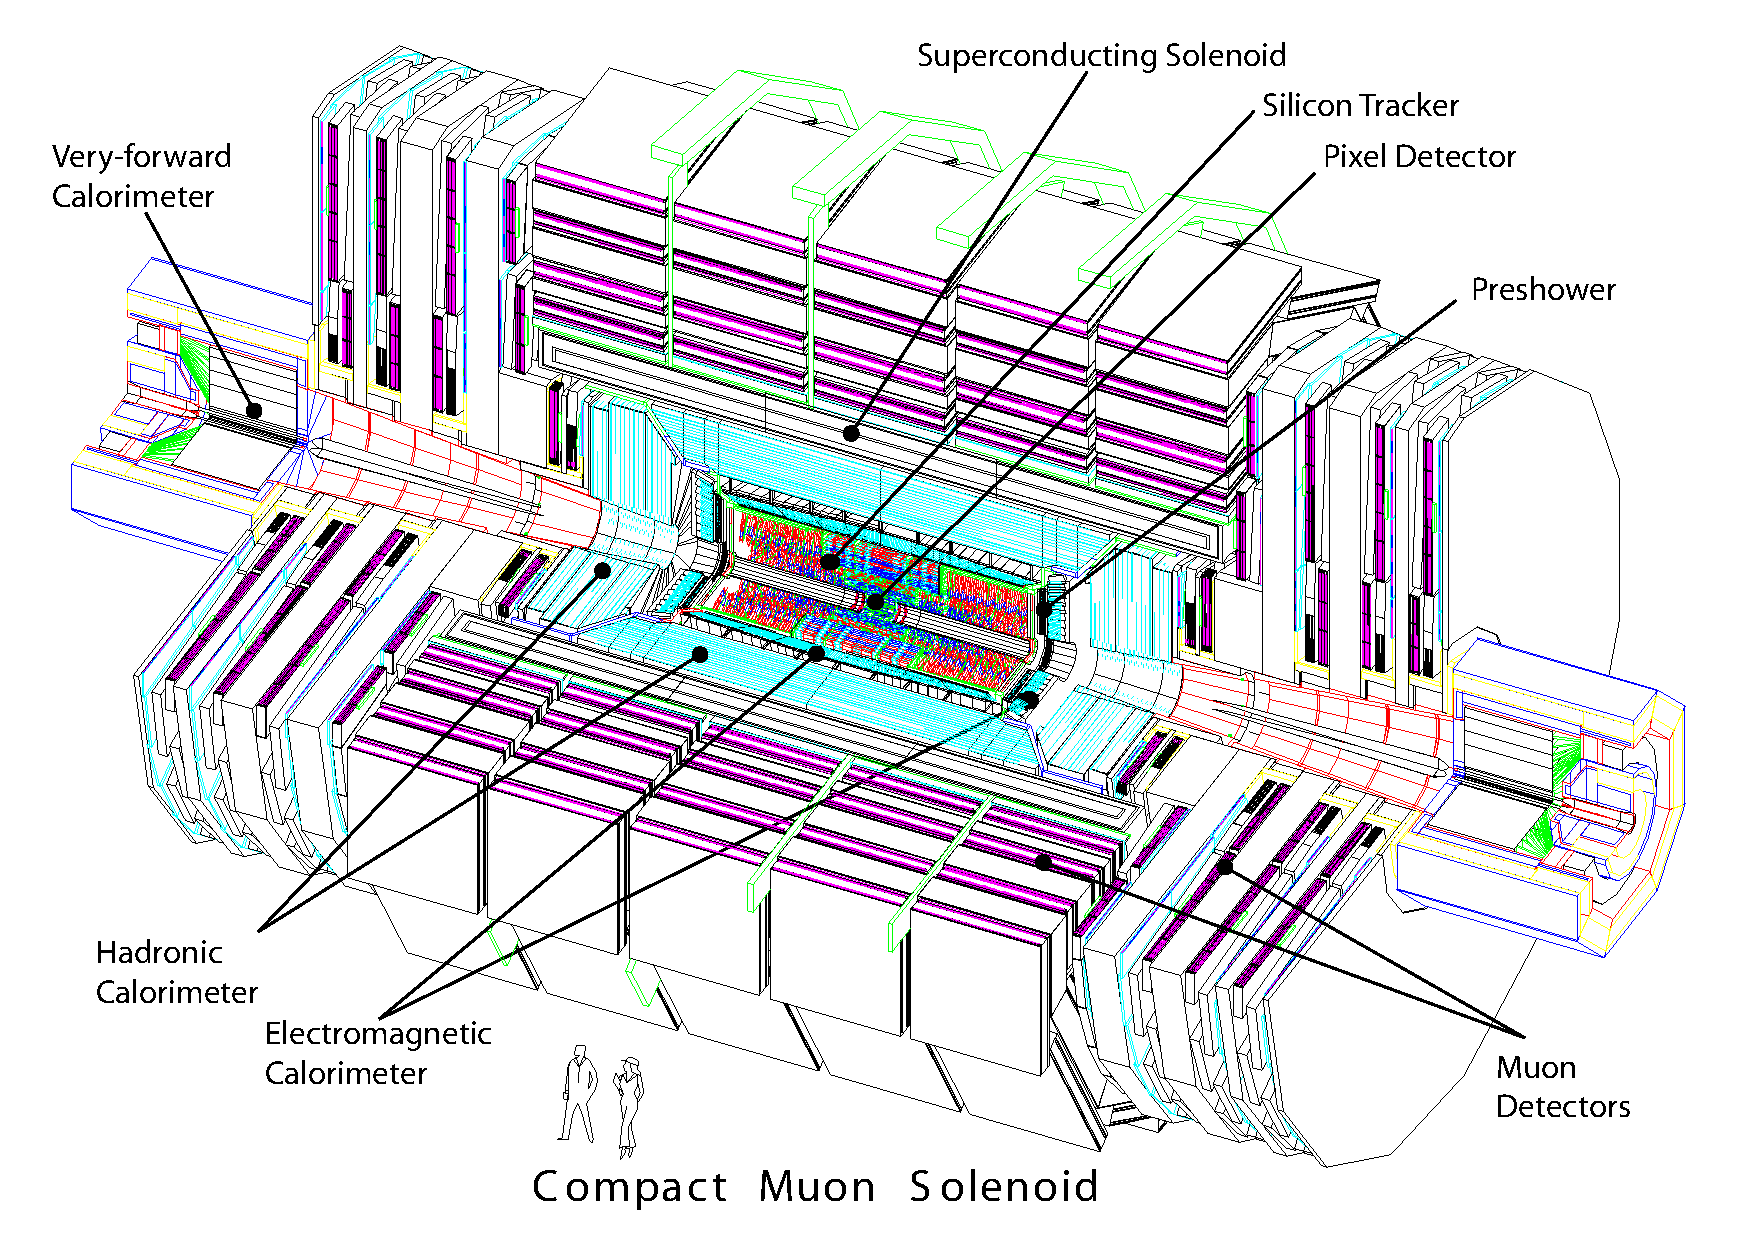
\includegraphics[width=0.7\textwidth]{Images/CMS_Layout.pdf}
\caption{CMS detector overview.}
\label{CMS_Layout}
\end{figure}






